\documentclass{standalone}
\usepackage{tikz}
\usetikzlibrary{patterns, positioning}

\begin{document}
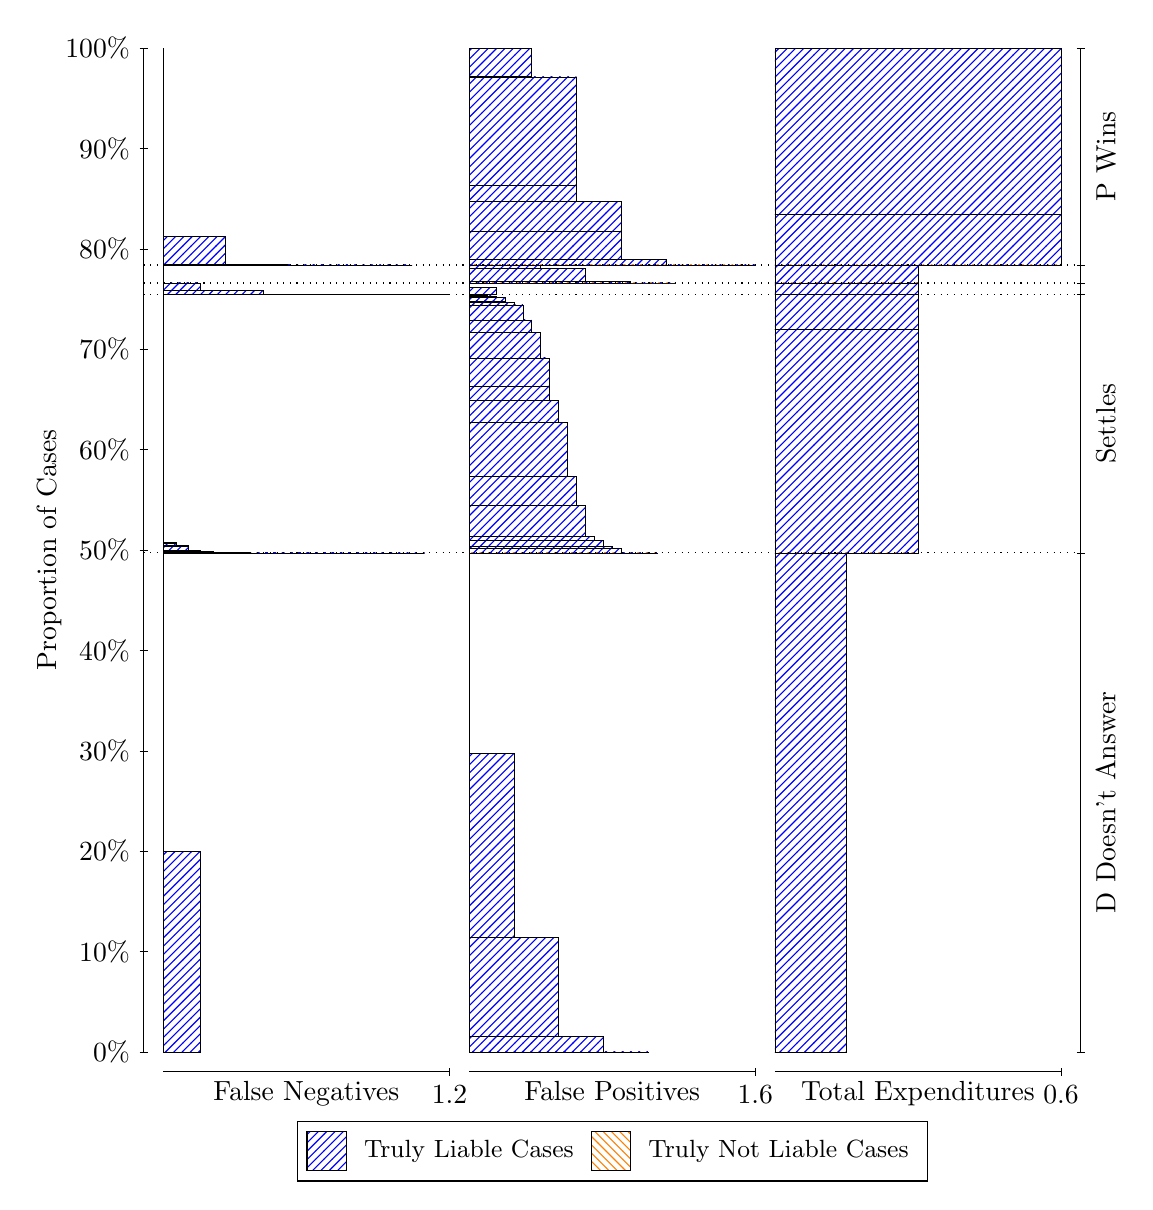
\begin{tikzpicture}
\draw[black, very thin] (1.5,1.75) -- (1.5,14.5);
\node[rotate=90, anchor=center] at (0.3, 8.125) {Proportion of Cases};
\draw[black, very thin] (1.45,1.75) -- (1.55,1.75);
\node[anchor=east] at (1.45, 1.75) {0\%};
\draw[black, very thin] (1.45,3.025) -- (1.55,3.025);
\node[anchor=east] at (1.45, 3.025) {10\%};
\draw[black, very thin] (1.45,4.3) -- (1.55,4.3);
\node[anchor=east] at (1.45, 4.3) {20\%};
\draw[black, very thin] (1.45,5.575) -- (1.55,5.575);
\node[anchor=east] at (1.45, 5.575) {30\%};
\draw[black, very thin] (1.45,6.85) -- (1.55,6.85);
\node[anchor=east] at (1.45, 6.85) {40\%};
\draw[black, very thin] (1.45,8.125) -- (1.55,8.125);
\node[anchor=east] at (1.45, 8.125) {50\%};
\draw[black, very thin] (1.45,9.4) -- (1.55,9.4);
\node[anchor=east] at (1.45, 9.4) {60\%};
\draw[black, very thin] (1.45,10.675) -- (1.55,10.675);
\node[anchor=east] at (1.45, 10.675) {70\%};
\draw[black, very thin] (1.45,11.95) -- (1.55,11.95);
\node[anchor=east] at (1.45, 11.95) {80\%};
\draw[black, very thin] (1.45,13.225) -- (1.55,13.225);
\node[anchor=east] at (1.45, 13.225) {90\%};
\draw[black, very thin] (1.45,14.5) -- (1.55,14.5);
\node[anchor=east] at (1.45, 14.5) {100\%};

\draw[black, very thin] (13.4,1.75) -- (13.4,14.5);
\draw[black, very thin] (13.35,1.75) -- (13.45,1.75);
\node[anchor=west] at (13.35, 1.75) {};
\draw[black, very thin] (13.35,8.089) -- (13.45,8.089);
\node[anchor=west] at (13.35, 8.089) {};
\draw[black, very thin] (13.35,11.369) -- (13.45,11.369);
\node[anchor=west] at (13.35, 11.369) {};
\draw[black, very thin] (13.35,11.516) -- (13.45,11.516);
\node[anchor=west] at (13.35, 11.516) {};
\draw[black, very thin] (13.35,11.745) -- (13.45,11.745);
\node[anchor=west] at (13.35, 11.745) {};
\draw[black, very thin] (13.35,14.5) -- (13.45,14.5);
\node[anchor=west] at (13.35, 14.5) {};

\draw[black, very thin, pattern color=blue, pattern=north east lines] (1.75,1.75) rectangle (2.2239,4.2978);
\draw[black, very thin, pattern color=orange, pattern=north west lines] (1.75,4.2978) rectangle (1.75,4.2978);
\draw[black, very thin, pattern color=blue, pattern=north east lines] (1.75,4.2978) rectangle (1.75,8.089);
\draw[black, very thin, pattern color=blue, pattern=north east lines] (1.75,8.089) rectangle (5.0674,8.089);
\draw[black, very thin, pattern color=blue, pattern=north east lines] (1.75,8.089) rectangle (4.7514,8.089);
\draw[black, very thin, pattern color=blue, pattern=north east lines] (1.75,8.089) rectangle (4.4355,8.089);
\draw[black, very thin, pattern color=blue, pattern=north east lines] (1.75,8.089) rectangle (4.2775,8.089);
\draw[black, very thin, pattern color=blue, pattern=north east lines] (1.75,8.089) rectangle (4.1196,8.089);
\draw[black, very thin, pattern color=blue, pattern=north east lines] (1.75,8.089) rectangle (3.9616,8.089);
\draw[black, very thin, pattern color=blue, pattern=north east lines] (1.75,8.089) rectangle (3.8036,8.089);
\draw[black, very thin, pattern color=blue, pattern=north east lines] (1.75,8.089) rectangle (3.6457,8.089);
\draw[black, very thin, pattern color=blue, pattern=north east lines] (1.75,8.089) rectangle (3.4877,8.0892);
\draw[black, very thin, pattern color=blue, pattern=north east lines] (1.75,8.0892) rectangle (3.3297,8.0892);
\draw[black, very thin, pattern color=blue, pattern=north east lines] (1.75,8.0892) rectangle (3.1717,8.0892);
\draw[black, very thin, pattern color=blue, pattern=north east lines] (1.75,8.0892) rectangle (3.1717,8.0896);
\draw[black, very thin, pattern color=blue, pattern=north east lines] (1.75,8.0896) rectangle (3.0138,8.0897);
\draw[black, very thin, pattern color=blue, pattern=north east lines] (1.75,8.0897) rectangle (2.8558,8.0908);
\draw[black, very thin, pattern color=blue, pattern=north east lines] (1.75,8.0908) rectangle (2.6978,8.0911);
\draw[black, very thin, pattern color=blue, pattern=north east lines] (1.75,8.0911) rectangle (2.6978,8.0921);
\draw[black, very thin, pattern color=blue, pattern=north east lines] (1.75,8.0921) rectangle (2.5399,8.0953);
\draw[black, very thin, pattern color=blue, pattern=north east lines] (1.75,8.0953) rectangle (2.3819,8.1007);
\draw[black, very thin, pattern color=blue, pattern=north east lines] (1.75,8.1007) rectangle (2.3819,8.1056);
\draw[black, very thin, pattern color=blue, pattern=north east lines] (1.75,8.1056) rectangle (2.2239,8.1241);
\draw[black, very thin, pattern color=blue, pattern=north east lines] (1.75,8.1241) rectangle (2.0659,8.1691);
\draw[black, very thin, pattern color=blue, pattern=north east lines] (1.75,8.1691) rectangle (2.0659,8.1854);
\draw[black, very thin, pattern color=blue, pattern=north east lines] (1.75,8.1854) rectangle (1.908,8.214);
\draw[black, very thin, pattern color=blue, pattern=north east lines] (1.75,8.214) rectangle (1.908,8.2192);
\draw[black, very thin, pattern color=blue, pattern=north east lines] (1.75,8.2192) rectangle (1.75,8.228);
\draw[black, very thin, pattern color=orange, pattern=north west lines] (1.75,8.228) rectangle (1.75,8.228);
\draw[black, very thin, pattern color=blue, pattern=north east lines] (1.75,8.228) rectangle (1.75,11.369);
\draw[black, very thin, pattern color=blue, pattern=north east lines] (1.75,11.369) rectangle (5.3833,11.369);
\draw[black, very thin, pattern color=blue, pattern=north east lines] (1.75,11.369) rectangle (4.5935,11.369);
\draw[black, very thin, pattern color=blue, pattern=north east lines] (1.75,11.369) rectangle (3.8036,11.373);
\draw[black, very thin, pattern color=blue, pattern=north east lines] (1.75,11.373) rectangle (3.0138,11.421);
\draw[black, very thin, pattern color=blue, pattern=north east lines] (1.75,11.421) rectangle (2.2239,11.516);
\draw[black, very thin, pattern color=orange, pattern=north west lines] (1.75,11.516) rectangle (1.75,11.516);
\draw[black, very thin, pattern color=blue, pattern=north east lines] (1.75,11.516) rectangle (2.2239,11.516);
\draw[black, very thin, pattern color=orange, pattern=north west lines] (1.75,11.516) rectangle (1.75,11.516);
\draw[black, very thin, pattern color=blue, pattern=north east lines] (1.75,11.516) rectangle (1.75,11.745);
\draw[black, very thin, pattern color=blue, pattern=north east lines] (1.75,11.745) rectangle (4.9094,11.745);
\draw[black, very thin, pattern color=blue, pattern=north east lines] (1.75,11.745) rectangle (4.1196,11.745);
\draw[black, very thin, pattern color=blue, pattern=north east lines] (1.75,11.745) rectangle (3.3297,11.755);
\draw[black, very thin, pattern color=blue, pattern=north east lines] (1.75,11.755) rectangle (2.5399,12.112);
\draw[black, very thin, pattern color=orange, pattern=north west lines] (1.75,12.112) rectangle (1.75,12.112);
\draw[black, very thin, pattern color=blue, pattern=north east lines] (1.75,12.112) rectangle (1.75,14.5);
\draw[black, very thin, pattern color=orange, pattern=north west lines] (5.6333,1.75) rectangle (7.9042,1.75);
\draw[black, very thin, pattern color=blue, pattern=north east lines] (5.6333,1.75) rectangle (7.9042,1.752);
\draw[black, very thin, pattern color=blue, pattern=north east lines] (5.6333,1.752) rectangle (7.3365,1.9506);
\draw[black, very thin, pattern color=blue, pattern=north east lines] (5.6333,1.9506) rectangle (6.7687,3.2011);
\draw[black, very thin, pattern color=blue, pattern=north east lines] (5.6333,3.2011) rectangle (6.201,5.5412);
\draw[black, very thin, pattern color=blue, pattern=north east lines] (5.6333,5.5412) rectangle (5.6333,8.089);
\draw[black, very thin, pattern color=orange, pattern=north west lines] (5.6333,8.089) rectangle (8.0177,8.089);
\draw[black, very thin, pattern color=blue, pattern=north east lines] (5.6333,8.089) rectangle (8.0177,8.0891);
\draw[black, very thin, pattern color=orange, pattern=north west lines] (5.6333,8.0891) rectangle (7.7906,8.0891);
\draw[black, very thin, pattern color=blue, pattern=north east lines] (5.6333,8.0891) rectangle (7.7906,8.0894);
\draw[black, very thin, pattern color=orange, pattern=north west lines] (5.6333,8.0894) rectangle (7.5635,8.0894);
\draw[black, very thin, pattern color=blue, pattern=north east lines] (5.6333,8.0894) rectangle (7.5635,8.1423);
\draw[black, very thin, pattern color=blue, pattern=north east lines] (5.6333,8.1423) rectangle (7.45,8.1714);
\draw[black, very thin, pattern color=orange, pattern=north west lines] (5.6333,8.1714) rectangle (7.3365,8.1714);
\draw[black, very thin, pattern color=blue, pattern=north east lines] (5.6333,8.1714) rectangle (7.3365,8.2493);
\draw[black, very thin, pattern color=blue, pattern=north east lines] (5.6333,8.2493) rectangle (7.2229,8.3019);
\draw[black, very thin, pattern color=orange, pattern=north west lines] (5.6333,8.3019) rectangle (7.1094,8.3019);
\draw[black, very thin, pattern color=blue, pattern=north east lines] (5.6333,8.3019) rectangle (7.1094,8.6954);
\draw[black, very thin, pattern color=blue, pattern=north east lines] (5.6333,8.6954) rectangle (6.9958,9.0609);
\draw[black, very thin, pattern color=orange, pattern=north west lines] (5.6333,9.0609) rectangle (6.8823,9.0609);
\draw[black, very thin, pattern color=blue, pattern=north east lines] (5.6333,9.0609) rectangle (6.8823,9.7469);
\draw[black, very thin, pattern color=orange, pattern=north west lines] (5.6333,9.7469) rectangle (6.8823,9.7469);
\draw[black, very thin, pattern color=blue, pattern=north east lines] (5.6333,9.7469) rectangle (6.8823,9.7494);
\draw[black, very thin, pattern color=blue, pattern=north east lines] (5.6333,9.7494) rectangle (6.7687,10.025);
\draw[black, very thin, pattern color=blue, pattern=north east lines] (5.6333,10.025) rectangle (6.6552,10.203);
\draw[black, very thin, pattern color=orange, pattern=north west lines] (5.6333,10.203) rectangle (6.6552,10.203);
\draw[black, very thin, pattern color=blue, pattern=north east lines] (5.6333,10.203) rectangle (6.6552,10.566);
\draw[black, very thin, pattern color=blue, pattern=north east lines] (5.6333,10.566) rectangle (6.5417,10.887);
\draw[black, very thin, pattern color=orange, pattern=north west lines] (5.6333,10.887) rectangle (6.4281,10.887);
\draw[black, very thin, pattern color=blue, pattern=north east lines] (5.6333,10.887) rectangle (6.4281,11.048);
\draw[black, very thin, pattern color=blue, pattern=north east lines] (5.6333,11.048) rectangle (6.3146,11.23);
\draw[black, very thin, pattern color=blue, pattern=north east lines] (5.6333,11.23) rectangle (6.3146,11.239);
\draw[black, very thin, pattern color=orange, pattern=north west lines] (5.6333,11.239) rectangle (6.201,11.239);
\draw[black, very thin, pattern color=blue, pattern=north east lines] (5.6333,11.239) rectangle (6.201,11.273);
\draw[black, very thin, pattern color=blue, pattern=north east lines] (5.6333,11.273) rectangle (6.0875,11.289);
\draw[black, very thin, pattern color=blue, pattern=north east lines] (5.6333,11.289) rectangle (6.0875,11.334);
\draw[black, very thin, pattern color=blue, pattern=north east lines] (5.6333,11.334) rectangle (5.974,11.352);
\draw[black, very thin, pattern color=blue, pattern=north east lines] (5.6333,11.352) rectangle (5.8604,11.363);
\draw[black, very thin, pattern color=blue, pattern=north east lines] (5.6333,11.363) rectangle (5.7469,11.365);
\draw[black, very thin, pattern color=blue, pattern=north east lines] (5.6333,11.365) rectangle (5.7469,11.366);
\draw[black, very thin, pattern color=blue, pattern=north east lines] (5.6333,11.366) rectangle (5.6333,11.369);
\draw[black, very thin, pattern color=orange, pattern=north west lines] (5.6333,11.369) rectangle (5.974,11.369);
\draw[black, very thin, pattern color=blue, pattern=north east lines] (5.6333,11.369) rectangle (5.974,11.464);
\draw[black, very thin, pattern color=blue, pattern=north east lines] (5.6333,11.464) rectangle (5.6333,11.516);
\draw[black, very thin, pattern color=orange, pattern=north west lines] (5.6333,11.516) rectangle (8.2448,11.516);
\draw[black, very thin, pattern color=blue, pattern=north east lines] (5.6333,11.516) rectangle (8.2448,11.516);
\draw[black, very thin, pattern color=blue, pattern=north east lines] (5.6333,11.516) rectangle (7.6771,11.538);
\draw[black, very thin, pattern color=blue, pattern=north east lines] (5.6333,11.538) rectangle (7.1094,11.699);
\draw[black, very thin, pattern color=blue, pattern=north east lines] (5.6333,11.699) rectangle (6.5417,11.745);
\draw[black, very thin, pattern color=blue, pattern=north east lines] (5.6333,11.745) rectangle (5.974,11.745);
\draw[black, very thin, pattern color=orange, pattern=north west lines] (5.6333,11.745) rectangle (9.2667,11.745);
\draw[black, very thin, pattern color=blue, pattern=north east lines] (5.6333,11.745) rectangle (9.2667,11.745);
\draw[black, very thin, pattern color=orange, pattern=north west lines] (5.6333,11.745) rectangle (8.699,11.745);
\draw[black, very thin, pattern color=blue, pattern=north east lines] (5.6333,11.745) rectangle (8.699,11.747);
\draw[black, very thin, pattern color=orange, pattern=north west lines] (5.6333,11.747) rectangle (8.1313,11.747);
\draw[black, very thin, pattern color=blue, pattern=north east lines] (5.6333,11.747) rectangle (8.1313,11.817);
\draw[black, very thin, pattern color=blue, pattern=north east lines] (5.6333,11.817) rectangle (7.5635,12.175);
\draw[black, very thin, pattern color=orange, pattern=north west lines] (5.6333,12.175) rectangle (7.5635,12.175);
\draw[black, very thin, pattern color=blue, pattern=north east lines] (5.6333,12.175) rectangle (7.5635,12.551);
\draw[black, very thin, pattern color=blue, pattern=north east lines] (5.6333,12.551) rectangle (6.9958,12.757);
\draw[black, very thin, pattern color=orange, pattern=north west lines] (5.6333,12.757) rectangle (6.9958,12.757);
\draw[black, very thin, pattern color=blue, pattern=north east lines] (5.6333,12.757) rectangle (6.9958,14.133);
\draw[black, very thin, pattern color=blue, pattern=north east lines] (5.6333,14.133) rectangle (6.4281,14.138);
\draw[black, very thin, pattern color=blue, pattern=north east lines] (5.6333,14.138) rectangle (6.4281,14.491);
\draw[black, very thin, pattern color=blue, pattern=north east lines] (5.6333,14.491) rectangle (5.8604,14.491);
\draw[black, very thin, pattern color=blue, pattern=north east lines] (5.6333,14.491) rectangle (5.8604,14.5);
\draw[black, very thin, pattern color=blue, pattern=north east lines] (5.6333,14.5) rectangle (5.6333,14.5);
\draw[black, very thin, pattern color=orange, pattern=north west lines] (9.5167,1.75) rectangle (10.425,1.75);
\draw[black, very thin, pattern color=blue, pattern=north east lines] (9.5167,1.75) rectangle (10.425,8.089);
\draw[black, very thin, pattern color=orange, pattern=north west lines] (9.5167,8.089) rectangle (11.333,8.089);
\draw[black, very thin, pattern color=blue, pattern=north east lines] (9.5167,8.089) rectangle (11.333,10.925);
\draw[black, very thin, pattern color=orange, pattern=north west lines] (9.5167,10.925) rectangle (11.333,10.925);
\draw[black, very thin, pattern color=blue, pattern=north east lines] (9.5167,10.925) rectangle (11.333,10.931);
\draw[black, very thin, pattern color=orange, pattern=north west lines] (9.5167,10.931) rectangle (11.333,10.931);
\draw[black, very thin, pattern color=blue, pattern=north east lines] (9.5167,10.931) rectangle (11.333,11.369);
\draw[black, very thin, pattern color=orange, pattern=north west lines] (9.5167,11.369) rectangle (11.333,11.369);
\draw[black, very thin, pattern color=blue, pattern=north east lines] (9.5167,11.369) rectangle (11.333,11.516);
\draw[black, very thin, pattern color=orange, pattern=north west lines] (9.5167,11.516) rectangle (11.333,11.516);
\draw[black, very thin, pattern color=blue, pattern=north east lines] (9.5167,11.516) rectangle (11.333,11.745);
\draw[black, very thin, pattern color=orange, pattern=north west lines] (9.5167,11.745) rectangle (13.15,11.745);
\draw[black, very thin, pattern color=blue, pattern=north east lines] (9.5167,11.745) rectangle (13.15,12.385);
\draw[black, very thin, pattern color=orange, pattern=north west lines] (9.5167,12.385) rectangle (13.15,12.385);
\draw[black, very thin, pattern color=blue, pattern=north east lines] (9.5167,12.385) rectangle (13.15,14.5);
\draw[black, dotted] (1.5,8.089) -- (13.4,8.089);
\draw[black, dotted] (1.5,11.369) -- (13.4,11.369);
\draw[black, dotted] (1.5,11.516) -- (13.4,11.516);
\draw[black, dotted] (1.5,11.745) -- (13.4,11.745);
\draw[black, very thin] (1.75,1.5) -- (5.3833,1.5);
\node[anchor=north] at (3.5667, 1.5) {False Negatives};
\draw[black, very thin] (5.3833,1.45) -- (5.3833,1.55);
\node[anchor=north] at (5.3833, 1.45) {1.2};

\draw[black, very thin] (5.6333,1.5) -- (9.2667,1.5);
\node[anchor=north] at (7.45, 1.5) {False Positives};
\draw[black, very thin] (9.2667,1.45) -- (9.2667,1.55);
\node[anchor=north] at (9.2667, 1.45) {1.6};

\draw[black, very thin] (9.5167,1.5) -- (13.15,1.5);
\node[anchor=north] at (11.333, 1.5) {Total Expenditures};
\draw[black, very thin] (13.15,1.45) -- (13.15,1.55);
\node[anchor=north] at (13.15, 1.45) {0.6};

\node[black, centered, rotate=90] at (13.72, 4.9195) {D Doesn't Answer};
\node[black, centered, rotate=90] at (13.72, 9.729) {Settles};


\node[black, centered, rotate=90] at (13.72, 13.123) {P Wins};

\draw (7.449999999999999,1.5) node[draw=none] (baseCoordinate) {};
\begin{scope}[align=center]
        \matrix[scale=0.5, draw=black, below=0.5cm of baseCoordinate, nodes={draw}, column sep=0.1cm]{
            \node[rectangle, draw, minimum width=0.5cm, minimum height=0.5cm, pattern=north east lines, pattern color=blue] {}; &
            \node[draw=none, font=\small] (B) {Truly Liable Cases}; &
            \node[rectangle, draw, minimum width=0.5cm, minimum height=0.5cm, pattern=north west lines, pattern color=orange] {}; &
            \node[draw=none, font=\small] (B) {Truly Not Liable Cases}; \\
            };
\end{scope}

\end{tikzpicture}
\end{document}